\documentclass{beamer}
\usefonttheme[onlymath]{serif}
\usepackage[T1]{fontenc}
\usepackage[utf8]{inputenc}
\usepackage[english]{babel}
\usepackage{amsmath}
\usepackage{amssymb}
\usepackage{amsthm}
\usepackage{gensymb}
\usepackage{parskip}
\usepackage{mathtools}
\usepackage{listings}
\usepackage{hyperref}
\usepackage{graphicx}
\usepackage{color}
\usepackage{enumerate}
\usepackage{tikz}
\usetikzlibrary{calc}
\usetikzlibrary{positioning}
\usetikzlibrary{angles}
\usetikzlibrary{shapes}
\usetikzlibrary{arrows}
\usepackage{verbatim}
\usepackage{multicol}
\usepackage{array}
\usepackage{minted}
\parskip 0pt


\DeclareMathOperator{\lcm}{lcm}
\newcommand\floor[1]{\left\lfloor#1\right\rfloor}
\newcommand\ceil[1]{\left\lceil#1\right\rceil}
\newcommand\abs[1]{\left|#1\right|}
\newcommand\p[1]{\left(#1\right)}
\newcommand\sqp[1]{\left[#1\right]}
\newcommand\cp[1]{\left\{#1\right\}}
\newcommand\norm[1]{\left\lVert#1\right\rVert}
\renewcommand\Im{\operatorname{Im}}
\renewcommand\Re{\operatorname{Re}}

\usetheme{metropolis}
\definecolor{dark yellow}{rgb} {0.6,0.6,0.0}
\definecolor{dark green}{rgb} {0.0,0.6,0.0}

\graphicspath{{myndir/}}

\title{Dynamic programming}
\author{Arnar Bjarni \& Atli FF}
\institute{\href{http://ru.is/td}{School of Computer Science} \\[2pt] \href{http://ru.is}{Reykjavík University}}
\titlegraphic{\hfill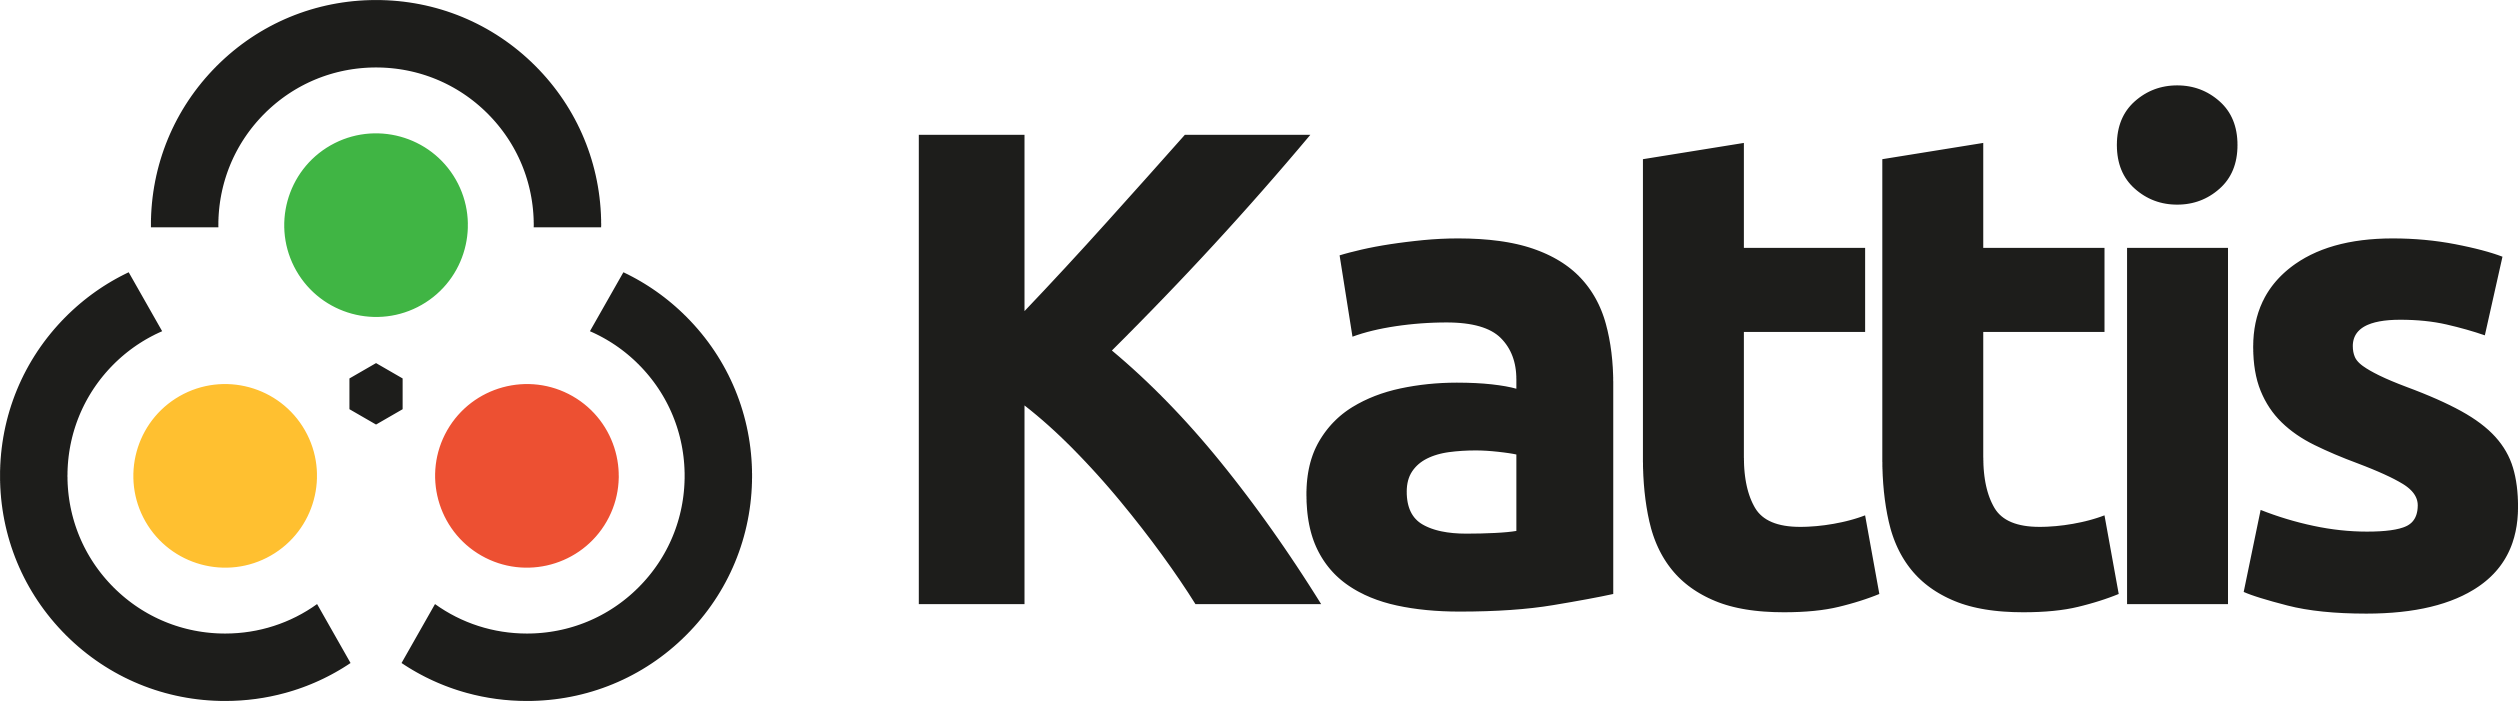
\includegraphics[height=0.6cm]{kattis}}

\begin{document}
\maketitle

\section*{Dynamic Programming}

\begin{frame}[plain]{What is dynamic programming?}
    \begin{itemize}
        \item A problem solving paradigm
        \item Similar in some respects to both divide and conquer and backtracking
        \vspace{5pt}
        \item Divide and conquer recap:
        \begin{itemize}
            \item Split the problem into \textit{independent} subproblems
            \item Solve each subproblem recursively
            \item Combine the solutions to subproblems into a solution for the given problem
        \end{itemize}
        \vspace{5pt}
        \item Dynamic programming:
        \begin{itemize}
            \item Split the problem into \textit{overlapping} subproblems
            \item Solve each subproblem recursively
            \item Combine the solutions to subproblems into a solution for the given problem
            \item \textit{Don't compute the answer to the same subproblem more than once}
        \end{itemize}
    \end{itemize}
\end{frame}

\begin{frame}[plain,fragile]{Dynamic programming formulation}
    \vspace{30pt}
    \begin{itemize}
        \item Formulate the problem in terms of smaller versions of the problem (recursively)
        \item Turn this formulation into a recursive function
        \item Memoize the function (remember results that have been computed)
    \end{itemize}
\end{frame}

\begin{frame}[plain,fragile]{Dynamic programming formulation}
    \begin{minted}[fontsize=\footnotesize]{cpp}
map<problem, value> memory;

value dp(problem P) {
    if (is_base_case(P)) {
        return base_case_value(P);
    }

    if (memory.find(P) != memory.end()) {
        return memory[P];
    }

    value result = some value;
    for (problem Q in subproblems(P)) {
        result = combine(result, dp(Q));
    }

    memory[P] = result;
    return result;
}
    \end{minted}
\end{frame}

\begin{frame}[plain]{The Fibonacci sequence}
    \vspace{5pt}
    \textit{The first two numbers in the Fibonacci sequence are 1 and 1. All
            other numbers in the sequence are defined as the sum of the previous two
            numbers in the sequence.}

    \vspace{5pt}
    \begin{itemize}
        \item Task: Find the $n$th number in the Fibonacci sequence
        \item Let's solve this with dynamic programming
    \end{itemize}

    \vspace{5pt}
    \begin{itemize}
        \item Formulate the problem in terms of smaller versions of the problem (recursively)
    \end{itemize}

    \begin{align*}
        \mathrm{fibonacci}(1) &= 1\\
        \mathrm{fibonacci}(2) &= 1\\
        \mathrm{fibonacci}(n) &= \mathrm{fibonacci}(n - 2) + \mathrm{fibonacci}(n - 1)
    \end{align*}
\end{frame}

\begin{frame}[plain,fragile]{The Fibonacci sequence}
    \begin{itemize}
        \item[2.] Turn this formulation into a recursive function
    \end{itemize}

    \begin{minted}[fontsize=\footnotesize]{cpp}
int fibonacci(int n) {
    if (n < 2) {
        return n;
    }

    int res = fibonacci(n - 2) + fibonacci(n - 1);

    return res;
}
    \end{minted}
\end{frame}

\begin{frame}[plain,fragile]{The Fibonacci sequence}
    \begin{itemize}
        \item What is the time complexity of this? \onslide<2->{Exponential, almost $O(2^n)$}
    \end{itemize}

    \begin{figure}

        \begin{tikzpicture}

[-,thick,%
  every node/.style={shape=circle,draw,thick},%
  level distance=0.5cm,
  growth parent anchor={south}, nodes={anchor=north},
  scale=0.8,%
]
\scriptsize
\node {$fib(6)$}
  [sibling distance=5cm]
  child {node {$fib(4)$}
    [sibling distance=2cm]
    child {node {$fib(2)$}
    }
    child {node {$fib(3)$}
      [sibling distance=1cm]
      child {node {$fib(1)$}
        [sibling distance=0.5cm]
      }
      child {node {$fib(2)$}
      }
    }
  }
  child {node {$fib(5)$}
    [sibling distance=3cm]
    child {node {$fib(3)$}
      [sibling distance=1cm]
      child {node {$fib(1)$}
        [sibling distance=0.5cm]
      }
      child {node {$fib(2)$}
          }
    }
    child {node {$fib(4)$}
      [sibling distance=2cm]
      child {node {$fib(2)$}
      }
      child {node {$fib(3)$}
        [sibling distance=1cm]
        child {node {$fib(1)$}
          [sibling distance=0.5cm]
        }
        child {node {$fib(2)$}
        }
      }
    }
  };
        \end{tikzpicture}
    \end{figure}
\end{frame}

\begin{frame}[plain,fragile]{The Fibonacci sequence}
    \begin{itemize}
        \item[3.] Memoize the function (remember results that have been computed)
    \end{itemize}

    \vspace{5pt}

    \begin{minted}[fontsize=\footnotesize]{cpp}
map<int, int> mem;

int fibonacci(int n) {
    if (n <= 2) {
        return 1;
    }

    if (mem.find(n) != mem.end()) {
        return mem[n];
    }

    int res = fibonacci(n - 2) + fibonacci(n - 1);

    mem[n] = res;
    return res;
}
    \end{minted}

\end{frame}

\begin{frame}[plain,fragile]{The Fibonacci sequence}
    \vspace{5pt}

    \begin{minted}[fontsize=\footnotesize]{cpp}
int mem[1000];
for (int i = 0; i < 1000; i++)
    mem[i] = -1;

int fibonacci(int n) {
    if (n <= 2) {
        return 1;
    }

    if (mem[n] != -1) {
        return mem[n];
    }

    int res = fibonacci(n - 2) + fibonacci(n - 1);

    mem[n] = res;
    return res;
}
    \end{minted}

\end{frame}

\begin{frame}[plain]{The Fibonacci sequence}
    \begin{itemize}
        \item What is the time complexity now?
        \vspace{5pt}
        \item We have $n$ possible inputs to the function: $1$, $2$, \ldots, $n$.
        \item Each input will either:
            \begin{itemize}
                \item be computed, and the result saved
                \item be returned from memory
            \end{itemize}
        \item Each input will be computed at most once
        \item Time complexity is $O(n \times f)$, where $f$ is the time complexity of computing an input if we assume that the recursive calls are returned directly from memory ($O(1)$)
        \item Since we're only doing constant amount of work to compute the answer to an input, $f = O(1)$
        \item Total time complexity is $O(n)$
    \end{itemize}
\end{frame}

\begin{frame}[plain]{Maximum sum}

    \vspace{10pt}

    \begin{itemize}
\item Given an array $\mathrm{arr}[0]$, $\mathrm{arr}[1]$, \ldots, $\mathrm{arr}[n-1]$ of integers, find the interval with the highest sum
    \end{itemize}

    \begin{center}
        \begin{tabular}{|c|c|c|c|c|c|c|}
            \hline
            -15 & \color<2->{blue}{8} & \color<2->{blue}{-2} & \color<2->{blue}{1} & \color<2->{blue}{0} & \color<2->{blue}{6} & -3 \\
            \hline
        \end{tabular}
    \end{center}

    \begin{itemize}
        \item<2-> The maximum sum of an interval in this array is $13$

        \item<3-> But how do we solve this in general?
            \begin{itemize}
        \item Easy to loop through all $\approx n^2$ intervals, and calculate their sums, but that is $O(n^3)$
        \item We could use our static range sum trick to get this down to $O(n^2)$
        \item Can we do better with dynamic programming?
            \end{itemize}
    \end{itemize}

\end{frame}

\begin{frame}[plain]{Maximum sum}

    \vspace{20pt}

    \begin{itemize}
        \item First step is to formulate this recursively
        \vspace{5pt}
        \item Let $\mathrm{max\_{}sum}(i)$ be the maximum sum interval in the range $0,\ldots,i$
        \vspace{5pt}
        \item Base case: $\mathrm{max\_{}sum}(0) = \mathrm{max}(0, arr[0])$
        \vspace{5pt}
        \item What about $\mathrm{max\_{}sum}(i)$?
        \item What does $\mathrm{max\_{}sum}(i-1)$ return?
        \item Is it possible to combine solutions to subproblems with smaller $i$ into a solution for $i$?
        \vspace{5pt}
        \item At least it's not obvious...
    \end{itemize}

\end{frame}

\begin{frame}[plain]{Maximum sum}

    \vspace{20pt}

    \begin{itemize}
        \item Let's try changing perspective
        \vspace{5pt}
    \item Let $\mathrm{max\_{}sum}(i)$ be the maximum sum interval in the range $0,\ldots,i$, \textit{that ends at $i$}
        \vspace{5pt}
        \item Base case: $\mathrm{max\_{}sum}(0) = arr[0]$
        \vspace{5pt}
    \item $\mathrm{max\_{}sum}(i) = \mathrm{max}(arr[i], arr[i] + \mathrm{max\_{}sum}(i - 1))$
        \vspace{15pt}
        \item Then the answer is just $\mathrm{max}_{\ 0 \leq i < n}\ \{\ \mathrm{max\_{}sum}(i)\ \}$
    \end{itemize}

\end{frame}

\begin{frame}[plain,fragile]{Maximum sum}
    \begin{itemize}
        \item Next step is to turn this into a function
    \end{itemize}

    \begin{minted}{cpp}
int arr[1000];

int max_sum(int i) {
    if (i == 0) {
        return arr[i];
    }

    int res = max(arr[i], arr[i] + max_sum(i - 1));

    return res;
}
    \end{minted}
\end{frame}

\begin{frame}[plain,fragile]{Maximum sum}
    \begin{itemize}
        \item Final step is to memoize the function
    \end{itemize}

    \begin{minted}[fontsize=\scriptsize]{cpp}
int arr[1000];
int mem[1000];
bool comp[1000];
memset(comp, 0, sizeof(comp));

int max_sum(int i) {
    if (i == 0) {
        return arr[i];
    }
    if (comp[i]) {
        return mem[i];
    }

    int res = max(arr[i], arr[i] + max_sum(i - 1));

    mem[i] = res;
    comp[i] = true;
    return res;
}
    \end{minted}
\end{frame}

\begin{frame}[plain,fragile]{Maximum sum}
    \begin{itemize}
        \item Then the answer is just the maximum over all interval ends
    \end{itemize}

    \begin{minted}{cpp}
int maximum = 0;
for (int i = 0; i < n; i++) {
    maximum = max(maximum, max_sum(i));
}

printf("%d\n", maximum);
    \end{minted}
\end{frame}

\begin{frame}[plain,fragile]{Maximum sum}
    \vspace{40pt}
    \begin{itemize}
        \item If you want to find the maximum sum interval in multiple arrays, remember to clear the memory in between
    \end{itemize}
\end{frame}

\begin{frame}[plain]{Maximum sum}
    \vspace{20pt}
    \begin{itemize}
        \item What about time complexity?
        \vspace{5pt}
        \item There are $n$ possible inputs to the function
        \item Each input is processed in $O(1)$ time, assuming recursive calls are $O(1)$
        \item Time complexity is $O(n)$
    \end{itemize}
\end{frame}

\begin{frame}[plain]{Coin change}
    \vspace{20pt}

    \begin{itemize}
\item Given an array of coin denominations $d_0$, $d_1$, \ldots, $d_{n-1}$,
            and some amount $x$: What is minimum number of coins needed to
            represent the value $x$?

        \item Remember the greedy algorithm for Coin change?
        \item It didn't always give the optimal solution, and sometimes it didn't even give a solution at all...

        \vspace{10pt}
        \item What about dynamic programming?
    \end{itemize}
\end{frame}

\begin{frame}[plain]{Coin change}
    \begin{itemize}
        \item First step: formulate the problem recursively
        \vspace{20pt}
\item Let $\mathrm{opt}(i,x)$ denote the minimum number of coins needed to represent the value $x$ if we're only allowed to use coin denominations $d_0$, \ldots, $d_i$
        \vspace{10pt}
        \item Base case: $\mathrm{opt}(i,x) = \infty$ if $x < 0$
        \item Base case: $\mathrm{opt}(i,0) = 0$
        \item Base case: $\mathrm{opt}(-1,x) = \infty$
        \vspace{10pt}
\item $\mathrm{opt}(i,x) = \mathrm{min} \left\{
	\begin{array}{l}
        1 + \mathrm{opt}(i, x - d_i) \\
        \mathrm{opt}(i-1, x)
	\end{array}
\right.$
    \end{itemize}
\end{frame}

\begin{frame}[plain,fragile]{Coin change}
    \begin{minted}[fontsize=\footnotesize]{cpp}
int INF = 100000;
int d[10];

int opt(int i, int x) {
    if (x < 0) return INF;
    if (x == 0) return 0;
    if (i == -1) return INF;

    int res = INF;
    res = min(res, 1 + opt(i, x - d[i]));
    res = min(res, opt(i - 1, x));

    return res;
}
    \end{minted}
\end{frame}

\begin{frame}[plain,fragile]{Coin change}
    \begin{minted}[fontsize=\footnotesize]{cpp}
int INF = 100000;
int d[10];
int mem[10][10000];
memset(mem, -1, sizeof(mem));

int opt(int i, int x) {
    if (x < 0) return INF;
    if (x == 0) return 0;
    if (i == -1) return INF;

    if (mem[i][x] != -1) return mem[i][x];

    int res = INF;
    res = min(res, 1 + opt(i, x - d[i]));
    res = min(res, opt(i - 1, x));

    mem[i][x] = res;
    return res;
}
    \end{minted}
\end{frame}

\begin{frame}[plain]{Coin change}
    \vspace{30pt}
    \begin{itemize}
        \item Time complexity?
        \item Number of possible inputs are $n \times x$
        \item Each input will be processed in $O(1)$ time, assuming recursive calls are constant
        \item Total time complexity is $O(n\times x)$
    \end{itemize}
\end{frame}

\begin{frame}[plain]{Coin change}
    \begin{itemize}
        \vspace{30pt}
        \item How do we know which coins the optimal solution used?
        \item We can store backpointers, or some extra information, to trace backwards through the states
        \item See example...
    \end{itemize}
\end{frame}

\begin{frame}[plain]{Longest increasing subsequence}
    \begin{itemize}
\item Given an array $a[0]$, $a[1]$, \ldots, $a[n-1]$ of integers, what is the length of the longest increasing subsequence?
    \vspace{5pt}
\item First, what is a subsequence?
\item If we delete zero or more elements from $a$, then we have a subsequence of $a$
    \vspace{5pt}
\item Example: $a = [5,1,8,1,9,2]$
    \vspace{5pt}
\item $[5,8,9]$ is a subsequence
\item $[1,1]$ is a subsequence
\item $[5,1,8,1,9,2]$ is a subsequence
\item $[]$ is a subsequence
\item $[8,5]$ is \textbf{not} a subsequence
\item $[10]$ is \textbf{not} a subsequence
    \end{itemize}
\end{frame}

\begin{frame}[plain]{Longest increasing subsequence}
    \begin{itemize}
\item Given an array $a[0]$, $a[1]$, \ldots, $a[n-1]$ of integers, what is the length of the longest increasing subsequence?
    \vspace{5pt}
\item An increasing subsequence of $a$ is a subsequence of $a$ such that the elements are in (strictly) increasing order
    \vspace{5pt}
\item $[5,8,9]$ and $[1,8,9]$ are the longest increasing subsequences of $a = [5,1,8,1,9,2]$

    \vspace{5pt}
\item How do we compute the length of the longest increasing subsequence?
\item There are $2^n$ subsequences, so we can go through all of them
\item That would result in an $O(n2^n)$ algorithm, which can only handle $n\leq 23$
    \vspace{5pt}
\item What about dynamic programming?

    \end{itemize}
\end{frame}

\begin{frame}[plain]{Longest increasing subsequence}
    \vspace{20pt}
    \begin{itemize}
\item Let $\mathrm{lis}(i)$ denote the length of the longest increasing subsequence of the array $a[0]$, $\ldots$, $a[i]$
    \vspace{5pt}
\item Base case: $\mathrm{lis}(0) = 1$
\item What about $\mathrm{lis}(i)$?
    \vspace{10pt}
\item We have the same issue as in the maximum sum problem, so let's try changing perspective
    \end{itemize}
\end{frame}

\begin{frame}[plain]{Longest increasing subsequence}
    \vspace{40pt}
    \begin{itemize}
\item Let $\mathrm{lis}(i)$ denote the length of the longest increasing subsequence of the array $a[0]$, $\ldots$, $a[i]$, \textit{that ends at $i$}
    \vspace{5pt}
\item Base case: we don't need one
\item $\mathrm{lis}(i) = \mathrm{max}(1, \mathrm{max}_{j<i \textrm{ s.t. } a[j] < a[i]} \{ 1 + \mathrm{lis}(j) \})$
    \end{itemize}
\end{frame}

\begin{frame}[plain,fragile]{Longest increasing subsequence}
    \begin{minted}[fontsize=\footnotesize]{cpp}
int a[1000];
int mem[1000];
memset(mem, -1, sizeof(mem));

int lis(int i) {
    if (mem[i] != -1) {
        return mem[i];
    }

    int res = 1;
    for (int j = 0; j < i; j++) {
        if (a[j] < a[i]) {
            res = max(res, 1 + lis(j));
        }
    }

    mem[i] = res;
    return res;
}
    \end{minted}
\end{frame}

\begin{frame}[plain,fragile]{Longest increasing subsequence}
    \vspace{30pt}

    \begin{itemize}
        \item And then the longest increasing subsequence can be found by checking all endpoints:
    \end{itemize}

    \begin{minted}{cpp}
int mx = 0;
for (int i = 0; i < n; i++) {
    mx = max(mx, lis(i));
}

printf("%d\n", mx);
    \end{minted}
\end{frame}

\begin{frame}[plain]{Longest increasing subsequence}
    \vspace{30pt}
    \begin{itemize}
        \item Time complexity?
            \vspace{10pt}
        \item There are $n$ possible inputs
        \item Each input is computed in $O(n)$ time, assuming recursive calls are $O(1)$
        \item Total time complexity is $O(n^2)$
            \vspace{10pt}
        \item This will be fast enough for $n \leq 10\ 000$, much better than the brute force method!
        \item (It can be done faster ($\mathcal{O}(n\log(n))$) with dynamic programming optimizations, but we're not covering that right now)
    \end{itemize}
\end{frame}


\begin{frame}[plain]{Longest common subsequence}
    \vspace{20pt}
    \begin{itemize}
\item Given two strings (or arrays of integers) $a[0]$, \ldots, $a[n-1]$ and $b[0]$, \ldots, $b[m-1]$, find the length of the longest subsequence that they have in common.

    \vspace{10pt}
\item $a = $\texttt{"b\underline{an}an\underline{inn}"}
\item $b = $\texttt{"k\underline{anin}a\underline{n}"}
    \vspace{5pt}
\item The longest common subsequence of $a$ and $b$, \texttt{"aninn"}, has length 5
    \end{itemize}
\end{frame}

\begin{frame}[plain]{Longest common subsequence}
    \vspace{20pt}
    \begin{itemize}
\item Let $\mathrm{lcs}(i, j)$ be the length of the longest common subsequence of the strings $a[0]$, \ldots, $a[i]$ and $b[0]$, \ldots, $b[j]$

    \vspace{10pt}
\item Base case: $\mathrm{lcs}(-1, j) = 0$
\item Base case: $\mathrm{lcs}(i, -1) = 0$
    \vspace{10pt}
\item $\mathrm{lcs}(i, j) = \mathrm{max} \left\{
	\begin{array}{ll}
        \mathrm{lcs}(i,j-1) & \\
        \mathrm{lcs}(i-1,j) & \\
        1 + \mathrm{lcs}(i-1,j-1) & \textrm{if } a[i] = b[j] \\
	\end{array}
\right.$
    \end{itemize}
\end{frame}

\begin{frame}[plain,fragile]{Longest common subsequence}
    \begin{minted}[fontsize=\scriptsize]{cpp}
string a = "bananinn",
       b = "kaninan";
int mem[1000][1000];
memset(mem, -1, sizeof(mem));

int lcs(int i, int j) {
    if (i == -1 || j == -1) {
        return 0;
    }
    if (mem[i][j] != -1) {
        return mem[i][j];
    }

    int res = 0;
    res = max(res, lcs(i, j - 1));
    res = max(res, lcs(i - 1, j));

    if (a[i] == b[j]) {
        res = max(res, 1 + lcs(i - 1, j - 1));
    }

    mem[i][j] = res;
    return res;
}
    \end{minted}
\end{frame}

\begin{frame}[plain]{Longest common subsequence}
    \vspace{40pt}
    \begin{itemize}
        \item Time complexity?
            \vspace{10pt}
        \item There are $n\times m$ possible inputs
        \item Each input is processed in $O(1)$, assuming recursive calls are $O(1)$
        \item Total time complexity is $O(n\times m)$
    \end{itemize}
\end{frame}

\begin{frame}[plain]{Coin Game}
    \begin{itemize}
        \item<1-> Two players play a game with a double ended queue of coins with different values.
        \item<1-> Take turns picking a coin from either end.
        \item<1-> Want to maximize total value at the end.
        \item<2-> Formulation: $\mathrm{dp}(i, j, p)$, solution is $\mathrm{dp}(0, n-1, 1)$.
        \item<2-> Base case when $i < j$: $\mathrm{dp}(i, j, p) = 0$
        \item<2-> Recursive step: \[
                \scriptstyle{\mathrm{dp}(i, j, p) = \mathrm{max}\left(p \cdot A_i + \mathrm{dp}(i+1, j, 1-p), p \cdot A_j + \mathrm{dp}(i, j-1, 1-p)\right)}
            \]
    \end{itemize}
\end{frame}

\begin{frame}[plain]{Narrow Art Gallery}
    \begin{itemize}
        \item We have a narrow art gallery, $N$ rows long and $2$ columns wide.
        \item Each cell has an exhibition of some value.
        \item Must close exactly $K$ exhibitions, still allowing people to pass through
        \item Goal is to maximize total value of open exhibitions
        \item What is our state?
        \item What information do we need to know our options?
    \end{itemize}
\end{frame}

\begin{frame}[plain]{Narrow Art Gallery}
    \begin{itemize}
        \item<1-> What is our state?
        \item<1-> What information do we need to know our options?
        \item<2-> Which row we are in
        \item<3-> How many we need to close
        \item<4-> What decision we made last time
    \end{itemize}
\end{frame}

\begin{frame}[plain]{Narrow Art Gallery}
    \begin{itemize}
        \item<1-> $\mathrm{dp}(i, k, c)$, where $i$ is remaining rows, $k$ is remaining to close and $c$ is our last choice
        \item<1-> $c = 0$ means close neither, $c = 1$ means close left, $c = 2$ means close right
        \item<2-> $\mathrm{dp}(0, 0, c) = 0$
        \item<2-> $\mathrm{dp}(0, k, c) = -\infty$ where $k \neq 0$
        \item<3-> $\mathrm{dp}(i, k, c) = \mathrm{max} \left\{
	\begin{array}{ll}
        A[i-1][0] + A[i-1][1] + \mathrm{dp}(i - 1, k, 0) & \\
        A[i-1][0] + \mathrm{dp}(i - 1, k - 1, 1) & \textrm{if } c \neq 2 \\
        A[i-1][1] + \mathrm{dp}(i - 1, k - 1, 2) & \textrm{if } c \neq 1 \\
	\end{array}
            \right\}.$
    \end{itemize}
\end{frame}

\begin{frame}[plain]{Top-down vs. bottom-up}
    \begin{itemize}
        \item What we have been doing so far is usually called top-down dynamic programming
        \item That is, you start with the main problem (the top) and split it into smaller problems recursively (down)
        \item In some cases it can be better to do things bottom-up, which is pretty much just the reverse order
        \item Consider for example the fibonacci numbers. Then we'd start at the base cases and count up
    \end{itemize}
\end{frame}

\begin{frame}[plain]{Top-down vs. bottom-up}
    \begin{itemize}
        \item Bottom-up is trickier to write, generally speaking. Top-down handles dependencies for us.
        \item Then why would we use bottom-up?
        \item Iteration is faster than recursion, so bottom-up is usually better performance
        \item Exception: Sparse DP computations.
        \item Sometimes there are optimizations which are easier to apply in bottom-up (later)
    \end{itemize}
\end{frame}

\end{document}
